%% arrowLength=10
%% linkWidth=3
%% input fy=50*node.pos
%% output fx=550
%% output fy=50*node.pos+25
%% MAX_FONT_SIZE=8
Imena razredov v glavah matrik zmot so okrajšana zaradi formatiranja dokumenta.
\begin{table}[H]
    \begin{center}
        \begin{tabular}{||l c c c||}
            \hline
            & 1        & 2        & 3 \\ [0.5ex]
            \hline
            velikost populacije              & 200      & 250      & 350      \\
            \hline
            največje število vmesnih vozlišč & 15       & 20       & 40       \\
            \hline
            največje število povezav         & 30       & 50       & 100      \\
            \hline
            največje število prečkanj        & 2        & 3        & 4        \\
            \hline
            delež mutiranih potomcev         & 10\%     & 10\%     & 10\%     \\
            \hline
            prispevek kompleksnosti          & -0.00001 & -0.00001 & -0.00001 \\
            \hline
            število generacij                & 200      & 250      & 300      \\
            \hline
        \end{tabular}
    \end{center}
    \caption{Nabori inicializacijskih parametrov poganjanja na množici Shuttle.}
    \label{tab:param_statlog}
\end{table}

\subsection{Prvi nabor}\label{subsec:dodatek-statlog-prvi-nabor}
%% branch shuttle
%% 200 15 30 2 true 0.1 100 true -0.00001 200 ACC
\begin{table}[H]
    \begin{center}
        \begin{tabular}{|| c | c c || c c ||}
            \hline
            \multirow{2}{*}{št. zagona} & \multicolumn{2}{c||}{točnost najboljšega agenta} & \multicolumn{2}{c||}{MKK najboljšega agenta} \\ \cline{2-5}
            & učna   & testna          & učna  & testna                  \\
            \hline
            1         & 91.6\% & 92.1\%          & 0.753 & 0.760                   \\
            \hline
            2         & 91.7\% & \textbf{92.2\%} & 0.750 & 0.758                   \\
            \hline
            3         & 91.7\% & 92.1\%          & 0.749 & 0.758                   \\
            \hline
            4         & 89.0\% & 89.5\%          & 0.749 & 0.756                   \\
            \hline
            5         & 89.3\% & 89.8\%          & 0.758 & \textbf{0.766 (92.2\%)} \\
            \hline
            povprečje & 90.7\% & 91.1\%          & 0.752 & 0.760                   \\
            \hline
            $\sigma$  & 0.012  & 0.012           & 0.003 & 0.003                   \\
            \hline
        \end{tabular}
    \end{center}
    \caption{Rezultat prvega nabora parametrov.}
    \label{tab:statlog_result_1}
\end{table}

\begin{table}[H]
    \centering
    \begin{tabular}{||rcccccccc||}
        \hline
        razred    & RF    & FC & FO & High & Bypass & BC & BO & vsota \\ \hline
        Rad Flow  & 11403 & 3  & 0  & 72   & 0      & 0  & 0  & 11478 \\ \hline
        Fpv Close & 1     & 10 & 0  & 2    & 0      & 0  & 0  & 13    \\ \hline
        Fpv Open  & 21    & 0  & 0  & 16   & 2      & 0  & 0  & 39    \\ \hline
        High      & 1006  & 0  & 0  & 1149 & 0      & 0  & 0  & 2155  \\ \hline
        Bypass    & 1     & 6  & 0  & 1    & 801    & 0  & 0  & 809   \\ \hline
        Bpv Close & 0     & 4  & 0  & 0    & 0      & 0  & 0  & 4     \\ \hline
        Bpv Open  & 2     & 0  & 0  & 0    & 0      & 0  & 0  & 2     \\ \hline
        vsota     & 12434 & 23 & 0  & 1240 & 803    & 0  & 0  & 14500 \\ \hline
    \end{tabular}
    \caption{Matrika zmot najbolj točnega agenta prvega nabora. Agent ne more napovedati razredov \enquote{Fpv Open}, \enquote{Bpv Close} in \enquote{Bpv Open}.}
    \label{tab:statlog_acc_1}
\end{table}

\begin{table}[H]
    \centering
    \begin{tabular}{||rcccccccc||}
        \hline
        razred    & RF    & FC & FO & High & Bypass & BC & BO & vsota \\ \hline
        Rad Flow  & 11442 & 1  & 2  & 33   & 0      & 0  & 0  & 11478 \\ \hline
        Fpv Close & 8     & 0  & 0  & 4    & 1      & 0  & 0  & 13    \\ \hline
        Fpv Open  & 24    & 0  & 0  & 13   & 1      & 0  & 1  & 39    \\ \hline
        High      & 1023  & 0  & 0  & 1132 & 0      & 0  & 0  & 2155  \\ \hline
        Bypass    & 0     & 1  & 3  & 4    & 800    & 0  & 1  & 809   \\ \hline
        Bpv Close & 1     & 0  & 0  & 3    & 0      & 0  & 0  & 4     \\ \hline
        Bpv Open  & 2     & 0  & 0  & 0    & 0      & 0  & 0  & 2     \\ \hline
        vsota     & 12500 & 2  & 5  & 1189 & 802    & 0  & 2  & 14500 \\ \hline
    \end{tabular}
    \caption{Matrika zmot agenta z največjim MKK prvega nabora. Agent ne more napovedati razreda \enquote{Bpv Close}.}
    \label{tab:statlog_mcc_1}
\end{table}

\begin{figure}[H]
    \begin{center}
        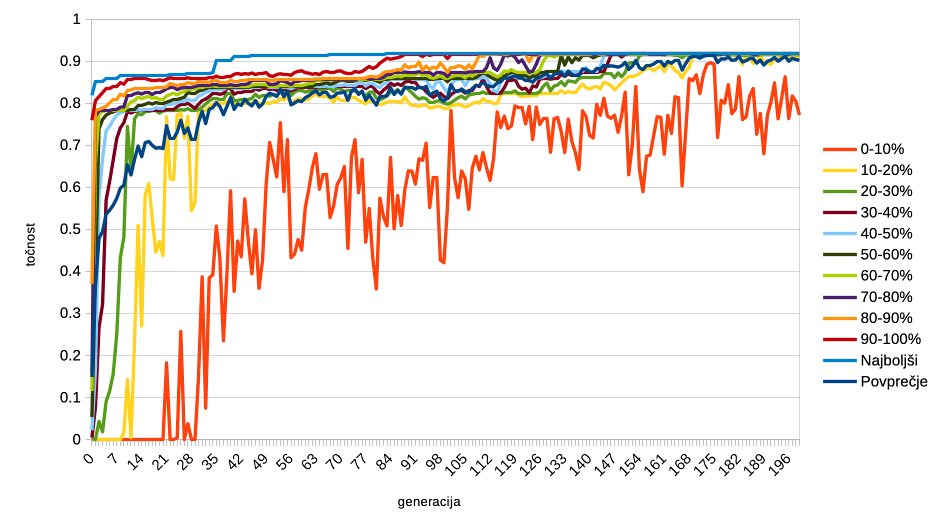
\includegraphics[width=13cm]{shuttle/1/acc}
    \end{center}
    \caption{Graf točnosti populacije najboljšega agenta prvega nabora skozi generacije.}
    \label{fig:statlog_acc_1}
\end{figure}

\begin{figure}[H]
    \begin{center}
        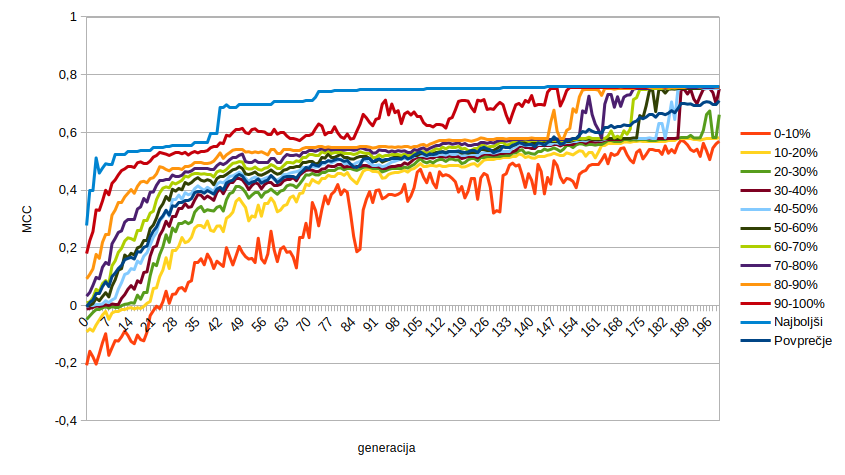
\includegraphics[width=13cm]{shuttle/1/mcc}
    \end{center}
    \caption{Graf MKK populacije najboljšega agenta prvega nabora skozi generacije.}
    \label{fig:statlog_mcc_1}
\end{figure}

\begin{figure}[H]
    \begin{center}
        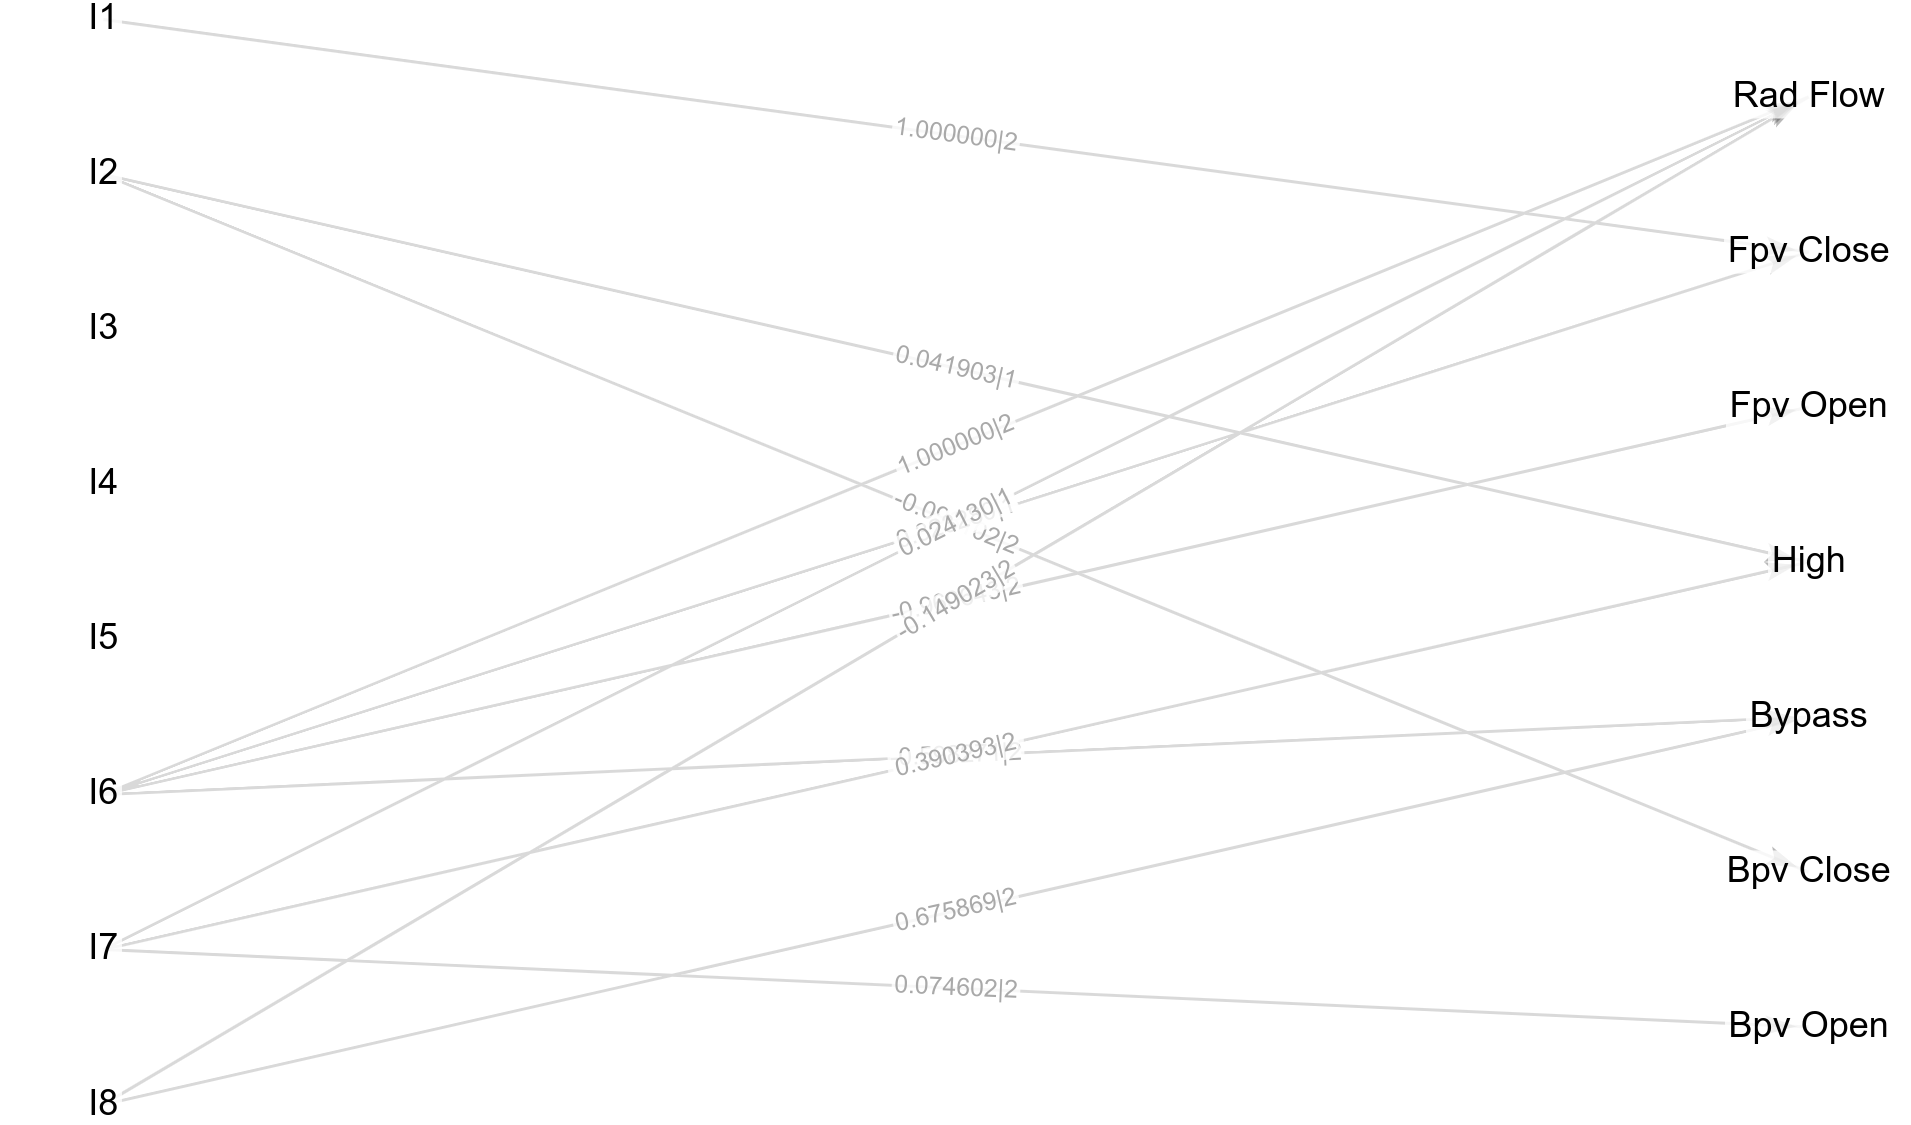
\includegraphics[width=13cm]{shuttle/1/acc_g}
    \end{center}
    \caption{Vizualizacija najbolj točnega agenta prvega nabora. Vsebuje 12 povezav.}
    \label{fig:statlog_acc_1_g}
\end{figure}

\begin{figure}[H]
    \begin{center}
        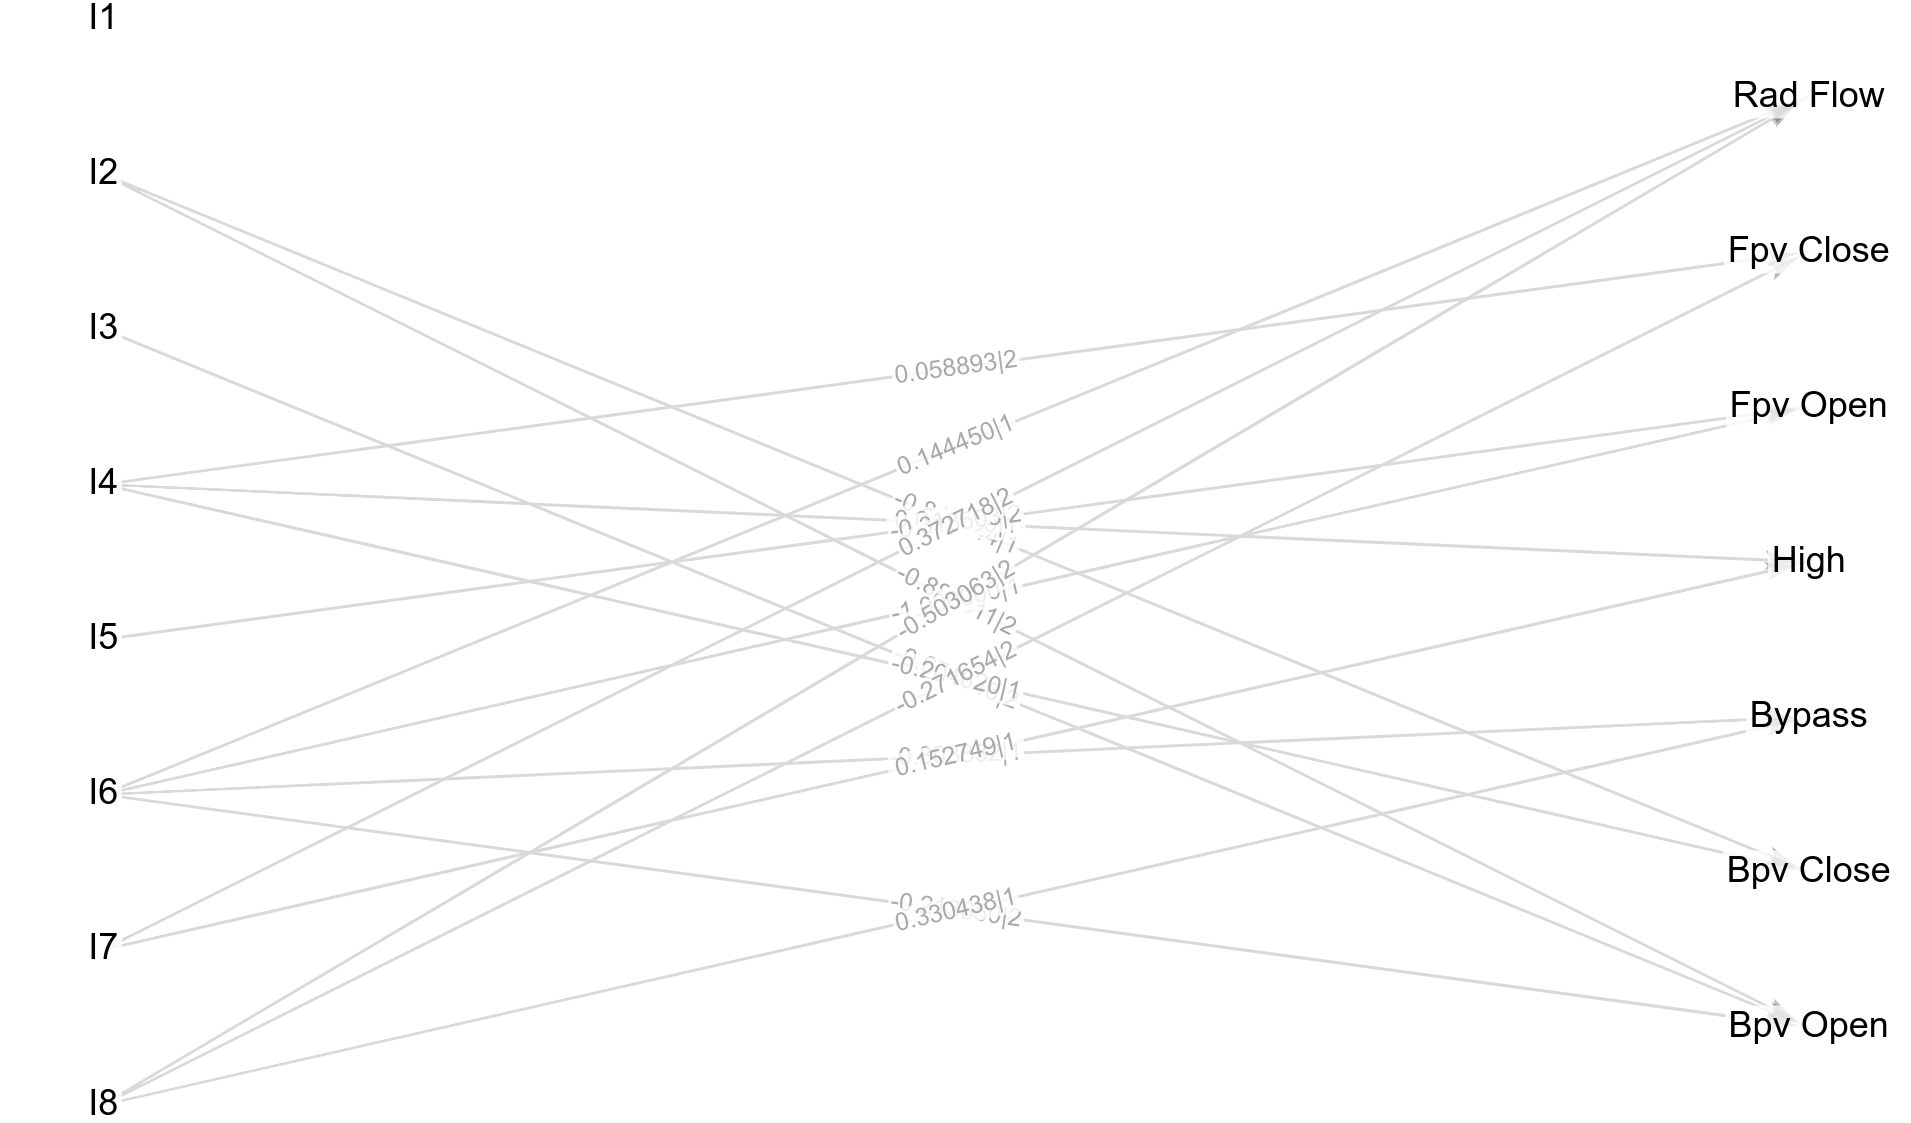
\includegraphics[width=13cm]{shuttle/1/mcc_g}
    \end{center}
    \caption{Vizualizacija agenta z največjim MKK prvega nabora. Vsebuje 16 povezav.}
    \label{fig:statlog_mcc_1_g}
\end{figure}

\subsection{Drugi nabor}\label{subsec:dodatek-statlog-drugi-nabor}
%% 250 20 50 3 true 0.1 125 true -0.00001 250 ACC
\begin{table}[H]
    \begin{center}
        \begin{tabular}{|| c | c c || c c ||}
            \hline
            \multirow{2}{*}{št. zagona} & \multicolumn{2}{c||}{točnost najboljšega agenta} & \multicolumn{2}{c||}{MKK najboljšega agenta} \\ \cline{2-5}
            & učna   & testna          & učna  & testna                  \\
            \hline
            1         & 87.6\% & 88.1\%          & 0.728 & 0.735                   \\
            \hline
            2         & 92.0\% & \textbf{92.4\%} & 0.600 & 0.604                   \\
            \hline
            3         & 86.4\% & 86.9\%          & 0.622 & 0.622                   \\
            \hline
            4         & 86.6\% & 87.1\%          & 0.767 & \textbf{0.774 (92.5\%)} \\
            \hline
            5         & 91.7\% & 92.2\%          & 0.755 & 0.761                   \\
            \hline
            povprečje & 88.9\% & 89.3\%          & 0.694 & 0.699                   \\
            \hline
            $\sigma$  & 0.025  & 0.022           & 0.070 & 0.072                   \\
            \hline
        \end{tabular}
    \end{center}
    \caption{Rezultat drugega nabora parametrov.}
    \label{tab:statlog_result_2}
\end{table}

\begin{table}[H]
    \centering
    \begin{tabular}{||rcccccccc||}
        \hline
        razred    & RF    & FC & FO & High & Bypass & BC & BO & vsota \\ \hline
        Rad Flow  & 11343 & 0  & 0  & 122  & 0      & 3  & 10 & 11478 \\ \hline
        Fpv Close & 5     & 0  & 0  & 8    & 0      & 0  & 0  & 13    \\ \hline
        Fpv Open  & 25    & 0  & 0  & 12   & 2      & 0  & 0  & 39    \\ \hline
        High      & 907   & 0  & 0  & 1248 & 0      & 0  & 0  & 2155  \\ \hline
        Bypass    & 0     & 0  & 0  & 0    & 805    & 3  & 1  & 809   \\ \hline
        Bpv Close & 0     & 0  & 0  & 3    & 1      & 0  & 0  & 4     \\ \hline
        Bpv Open  & 0     & 0  & 0  & 0    & 0      & 0  & 2  & 2     \\ \hline
        vsota     & 12280 & 0  & 0  & 1393 & 808    & 6  & 13 & 14500 \\ \hline
    \end{tabular}
    \caption{Matrika zmot najbolj točnega agenta drugega nabora. Agent ne more napovedati razredov \enquote{Fpv Close} in \enquote{Fpv Open}.}
    \label{tab:statlog_acc_2}
\end{table}

\begin{table}[H]
    \centering
    \begin{tabular}{||rcccccccc||}
        \hline
        razred    & RF    & FC & FO & High & Bypass & BC & BO & vsota \\ \hline
        Rad Flow  & 11416 & 0  & 1  & 51   & 0      & 4  & 6  & 11478 \\ \hline
        Fpv Close & 6     & 0  & 0  & 7    & 0      & 0  & 0  & 13    \\ \hline
        Fpv Open  & 17    & 1  & 0  & 21   & 0      & 0  & 0  & 39    \\ \hline
        High      & 954   & 0  & 0  & 1200 & 0      & 0  & 1  & 2155  \\ \hline
        Bypass    & 0     & 1  & 4  & 4    & 797    & 2  & 1  & 809   \\ \hline
        Bpv Close & 0     & 0  & 4  & 0    & 0      & 0  & 0  & 4     \\ \hline
        Bpv Open  & 2     & 0  & 0  & 0    & 0      & 0  & 0  & 2     \\ \hline
        vsota     & 12395 & 2  & 9  & 1283 & 797    & 6  & 8  & 14500 \\ \hline
    \end{tabular}
    \caption{Matrika zmot agenta z največjim MKK drugega nabora.}
    \label{tab:statlog_mcc_2}
\end{table}

\begin{figure}[H]
    \begin{center}
        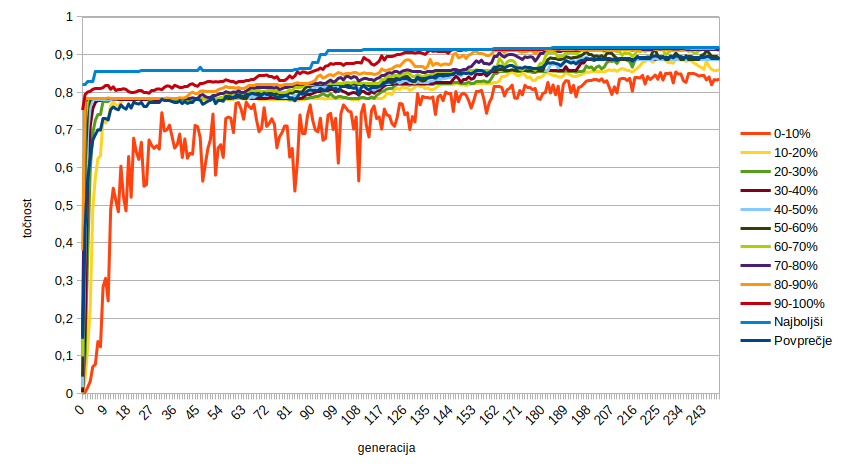
\includegraphics[width=13cm]{shuttle/2/acc}
    \end{center}
    \caption{Graf točnosti populacije najboljšega agenta drugega nabora skozi generacije.}
    \label{fig:statlog_acc_2}
\end{figure}

\begin{figure}[H]
    \begin{center}
        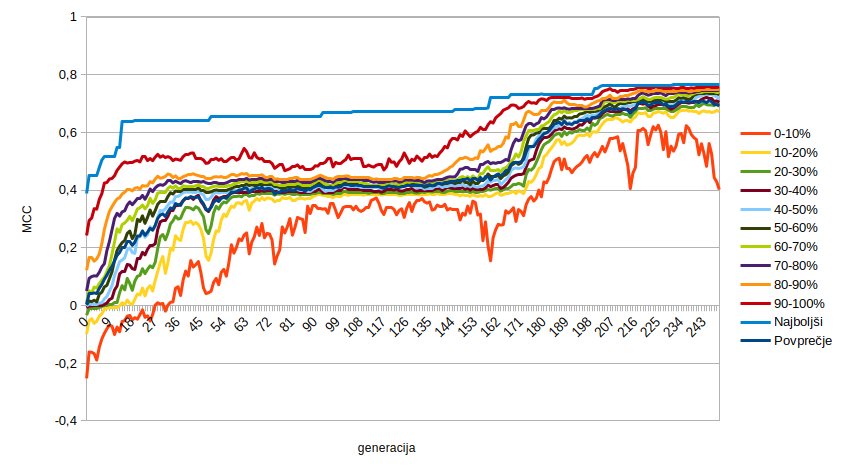
\includegraphics[width=13cm]{shuttle/2/mcc}
    \end{center}
    \caption{Graf MKK populacije najboljšega agenta drugega nabora skozi generacije.}
    \label{fig:statlog_mcc_2}
\end{figure}

\begin{figure}[H]
    \begin{center}
        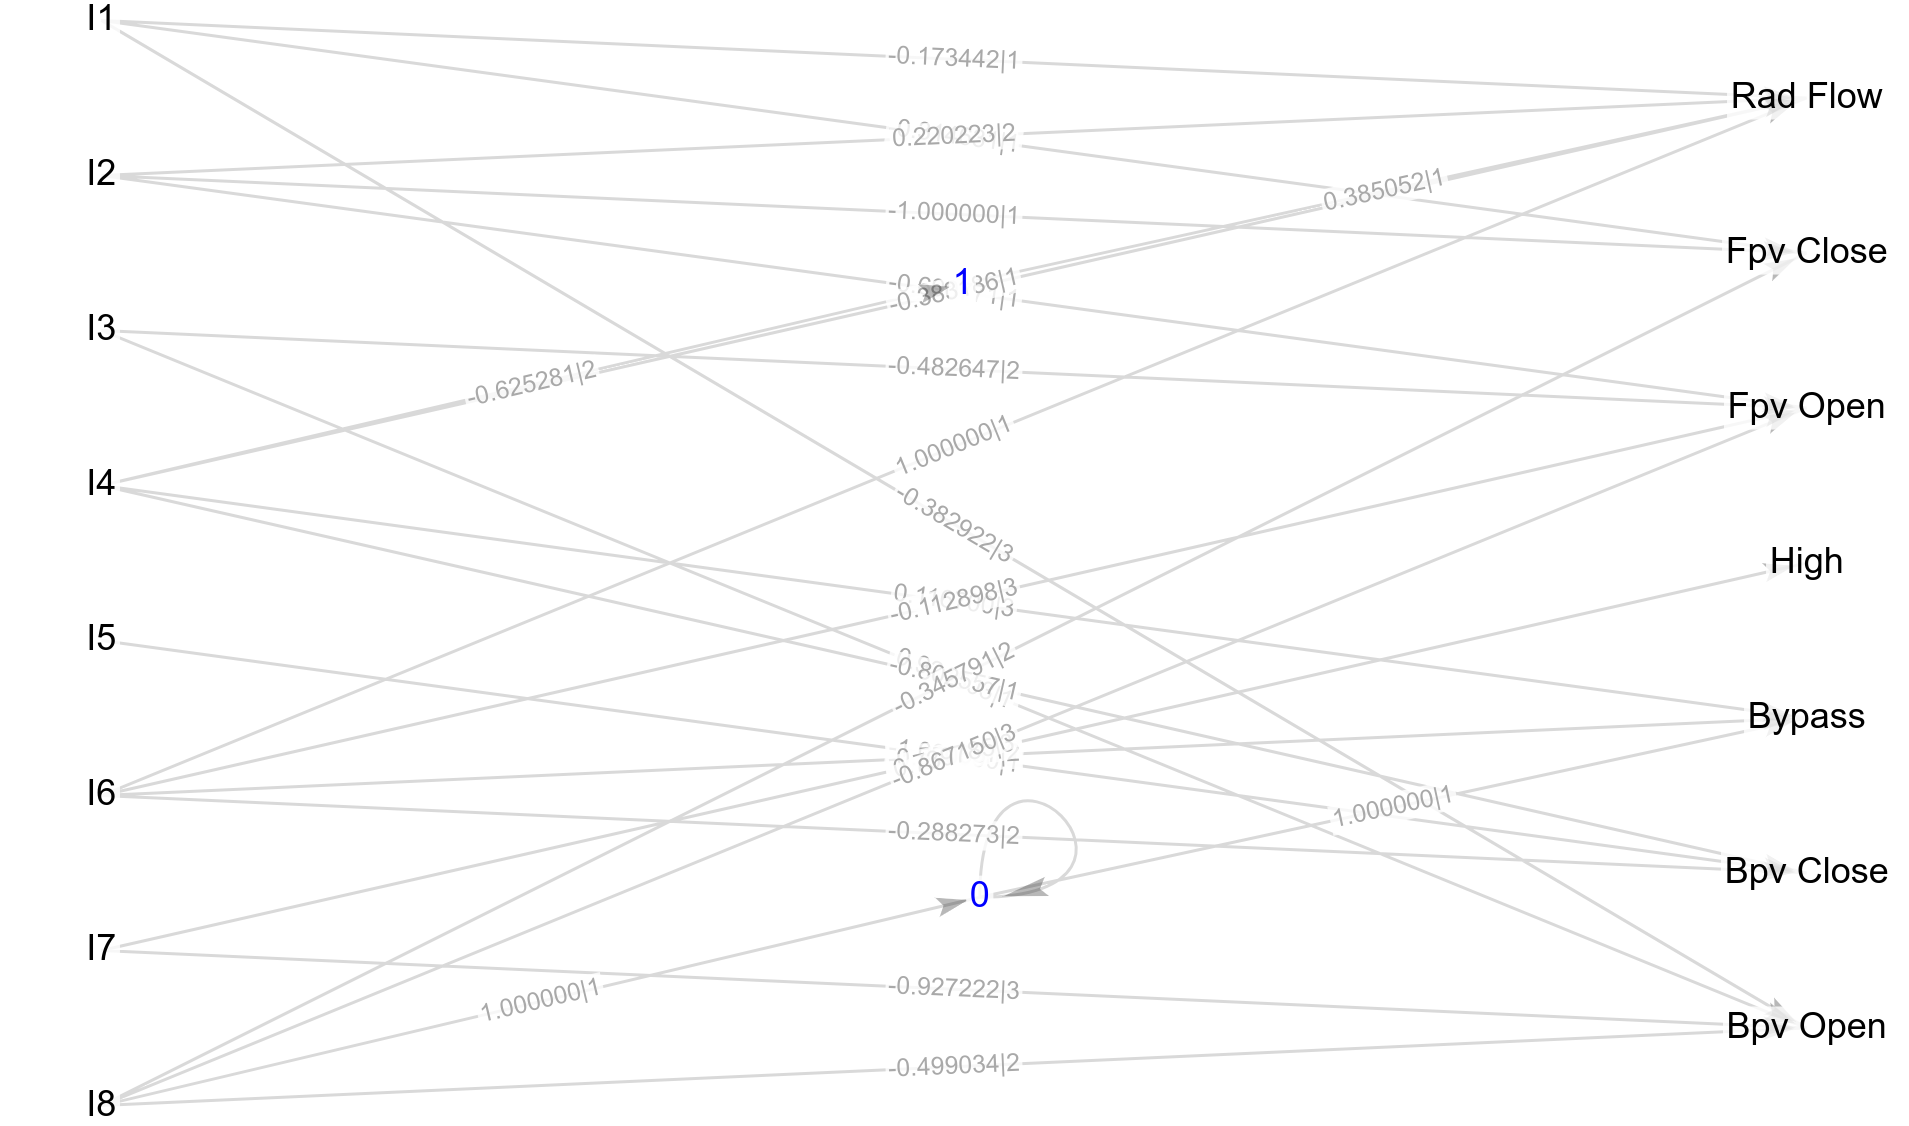
\includegraphics[width=13cm]{shuttle/2/acc_g}
    \end{center}
    \caption{Vizualizacija najbolj točnega agenta drugega nabora. Vsebuje 2 vmesni vozlišči in 26 povezav.}
    \label{fig:statlog_acc_2_g}
\end{figure}

\begin{figure}[H]
    \begin{center}
        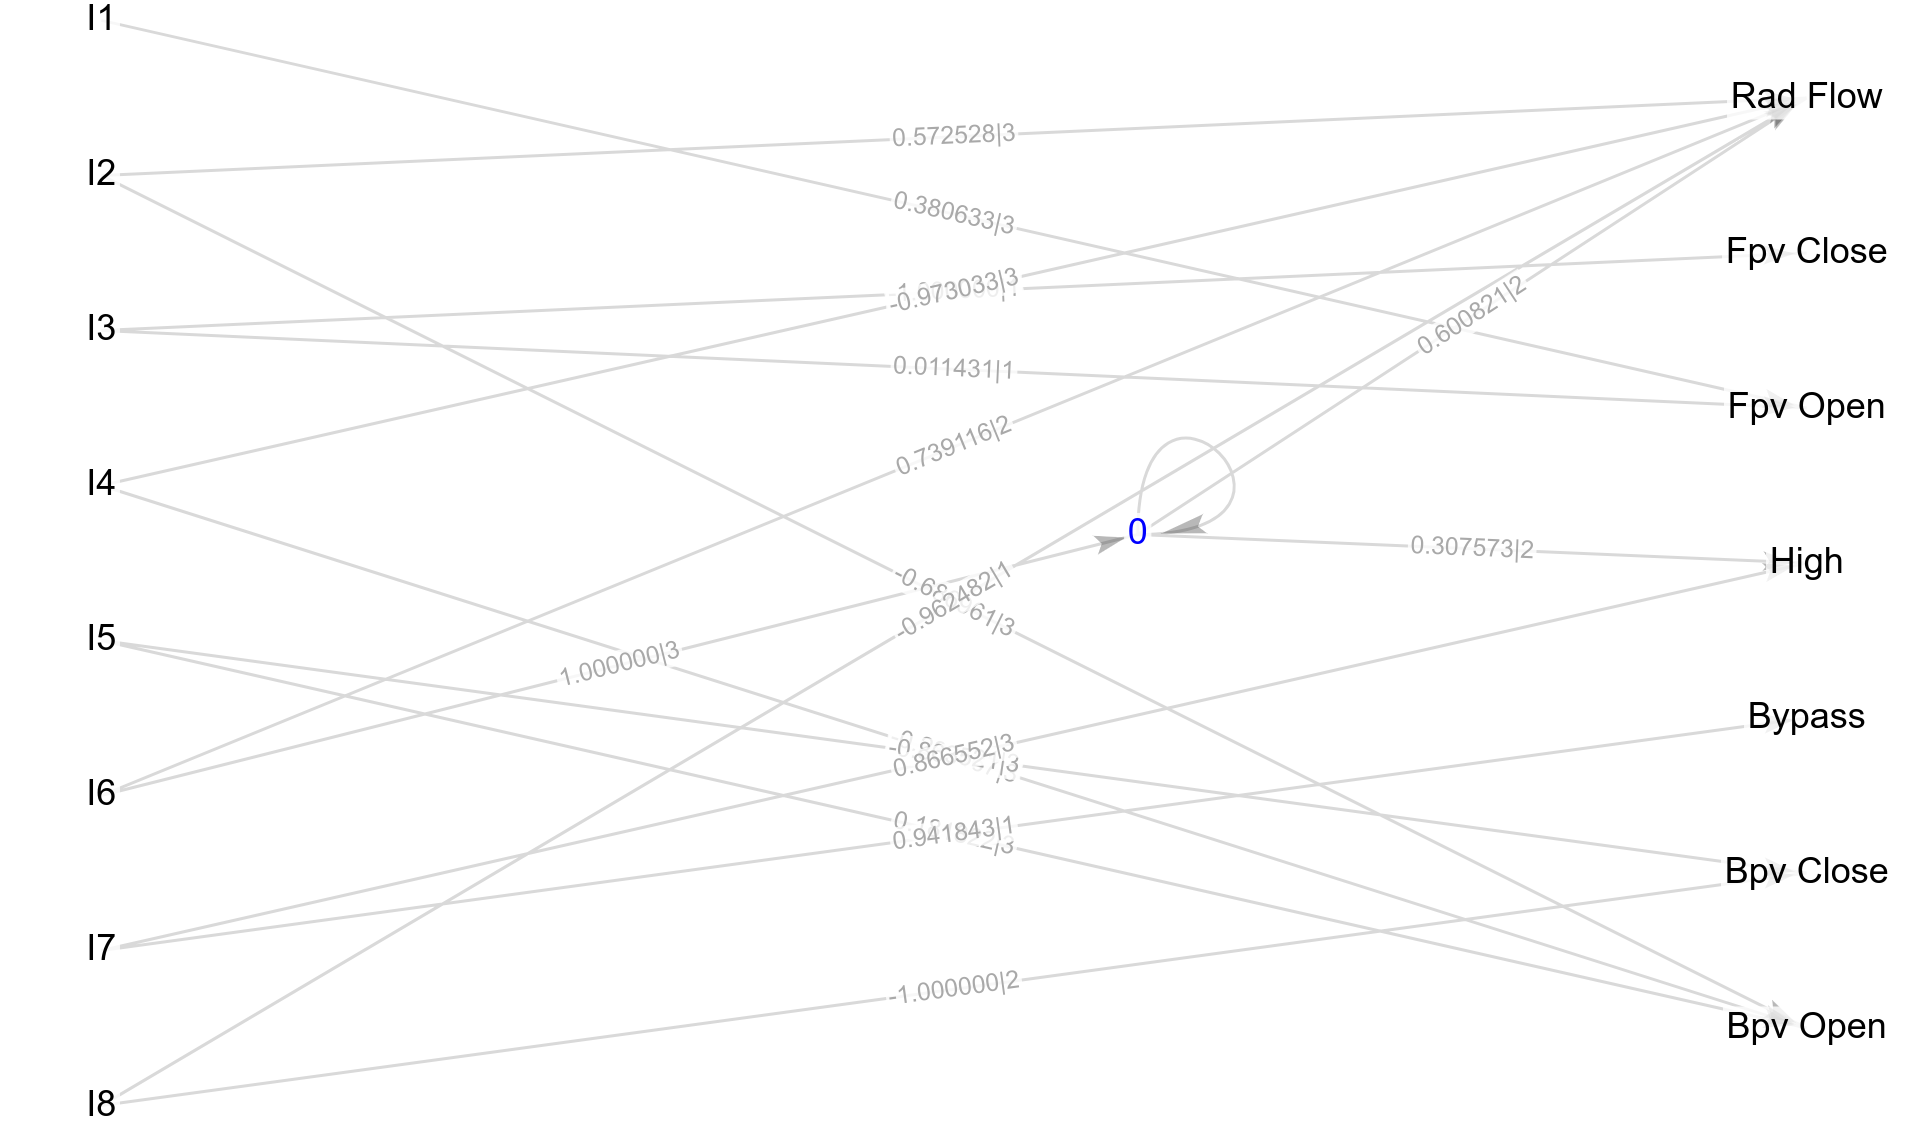
\includegraphics[width=13cm]{shuttle/2/mcc_g}
    \end{center}
    \caption{Vizualizacija agenta z največjim MKK drugega nabora. Vsebuje 1 vmesno vozlišče in 18 povezav.}
    \label{fig:statlog_mcc_2_g}
\end{figure}

\subsection{Tretji nabor}\label{subsec:dodatek-statlog-tretji-nabor}
%% 350 40 100 4 true 0.1 175 true -0.00001 300 ACC
\begin{table}[H]
    \begin{center}
        \begin{tabular}{|| c | c c || c c ||}
            \hline
            \multirow{2}{*}{št. zagona} & \multicolumn{2}{c||}{točnost najboljšega agenta} & \multicolumn{2}{c||}{MKK najboljšega agenta} \\ \cline{2-5}
            & učna   & testna          & učna  & testna                  \\
            \hline
            1         & 88.6\% & 89.2\%          & 0.755 & 0.762                   \\
            \hline
            2         & 92.6\% & \textbf{93.0\%} & 0.755 & 0.762                   \\
            \hline
            3         & 90.1\% & 90.6\%          & 0.749 & 0.757                   \\
            \hline
            4         & 88.0\% & 88.6\%          & 0.653 & 0.657                   \\
            \hline
            5         & 90.6\% & 91.0\%          & 0.785 & \textbf{0.790 (93.0\%)} \\
            \hline
            povprečje & 90.0\% & 90.5\%          & 0.739 & 0.746                   \\
            \hline
            $\sigma$  & 0.016  & 0.015           & 0.045 & 0.046                   \\
            \hline
        \end{tabular}
    \end{center}
    \caption{Rezultat tretjega nabora parametrov.}
    \label{tab:statlog_result_3}
\end{table}

\begin{table}[H]
    \centering
    \begin{tabular}{||rcccccccc||}
        \hline
        razred    & RF    & FC & FO & High & Bypass & BC & BO & vsota \\ \hline
        Rad Flow  & 11470 & 0  & 0  & 2    & 0      & 1  & 5  & 11478 \\ \hline
        Fpv Close & 6     & 0  & 0  & 7    & 0      & 0  & 0  & 13    \\ \hline
        Fpv Open  & 18    & 0  & 0  & 20   & 0      & 0  & 1  & 39    \\ \hline
        High      & 947   & 0  & 0  & 1208 & 0      & 0  & 0  & 2155  \\ \hline
        Bypass    & 0     & 0  & 0  & 0    & 807    & 3  & 2  & 809   \\ \hline
        Bpv Close & 1     & 0  & 0  & 3    & 0      & 0  & 0  & 4     \\ \hline
        Bpv Open  & 1     & 0  & 0  & 0    & 0      & 0  & 1  & 2     \\ \hline
        vsota     & 12443 & 0  & 0  & 1240 & 807    & 1  & 9  & 14500 \\ \hline
    \end{tabular}
    \caption{Matrika zmot najbolj točnega agenta tretjega nabora. Agent ne more napovedati razredov \enquote{Fpv Close} in \enquote{Fpv Open}.}
    \label{tab:statlog_acc_3}
\end{table}

\begin{table}[H]
    \centering
    \begin{tabular}{||rcccccccc||}
        \hline
        razred    & RF    & FC & FO & High & Bypass & BC & BO & vsota \\ \hline
        Rad Flow  & 11456 & 0  & 8  & 9    & 1      & 0  & 4  & 11478 \\ \hline
        Fpv Close & 6     & 0  & 0  & 4    & 3      & 0  & 0  & 13    \\ \hline
        Fpv Open  & 18    & 0  & 0  & 21   & 0      & 0  & 0  & 39    \\ \hline
        High      & 893   & 0  & 0  & 1262 & 0      & 0  & 0  & 2155  \\ \hline
        Bypass    & 0     & 0  & 1  & 41   & 767    & 0  & 0  & 809   \\ \hline
        Bpv Close & 0     & 0  & 0  & 0    & 4      & 0  & 0  & 4     \\ \hline
        Bpv Open  & 0     & 0  & 0  & 0    & 0      & 0  & 2  & 2     \\ \hline
        vsota     & 12373 & 0  & 9  & 1337 & 775    & 0  & 6  & 14500 \\ \hline
    \end{tabular}
    \caption{Matrika zmot agenta z največjim MKK tretjega nabora. Agent ne more napovedati razredov \enquote{Fpv Close} in \enquote{Bpv Close}.}
    \label{tab:statlog_mcc_3}
\end{table}

\begin{figure}[H]
    \begin{center}
        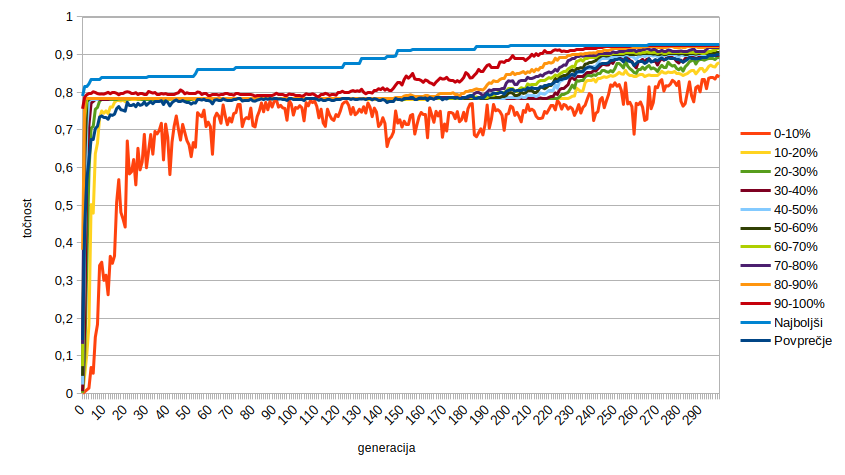
\includegraphics[width=13cm]{shuttle/3/acc}
    \end{center}
    \caption{Graf točnosti populacije najboljšega agenta tretjega nabora skozi generacije.}
    \label{fig:statlog_acc_3}
\end{figure}

\begin{figure}[H]
    \begin{center}
        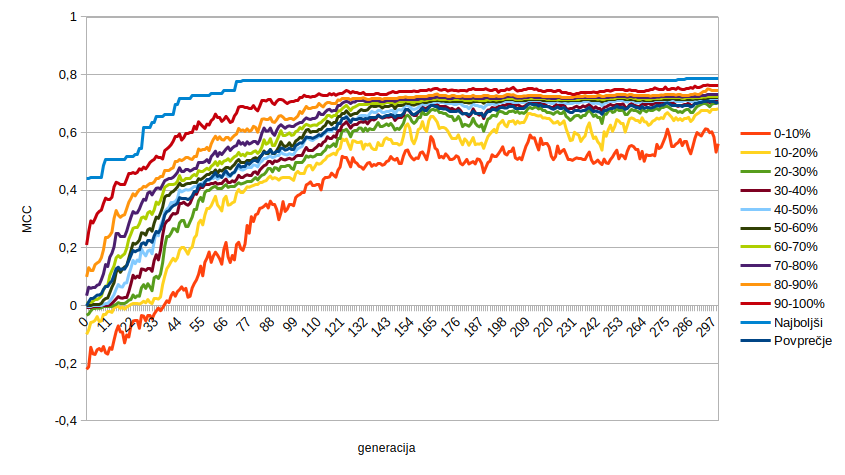
\includegraphics[width=13cm]{shuttle/3/mcc}
    \end{center}
    \caption{Graf MKK populacije najboljšega agenta tretjega nabora skozi generacije.}
    \label{fig:statlog_mcc_3}
\end{figure}

\begin{figure}[H]
    \begin{center}
        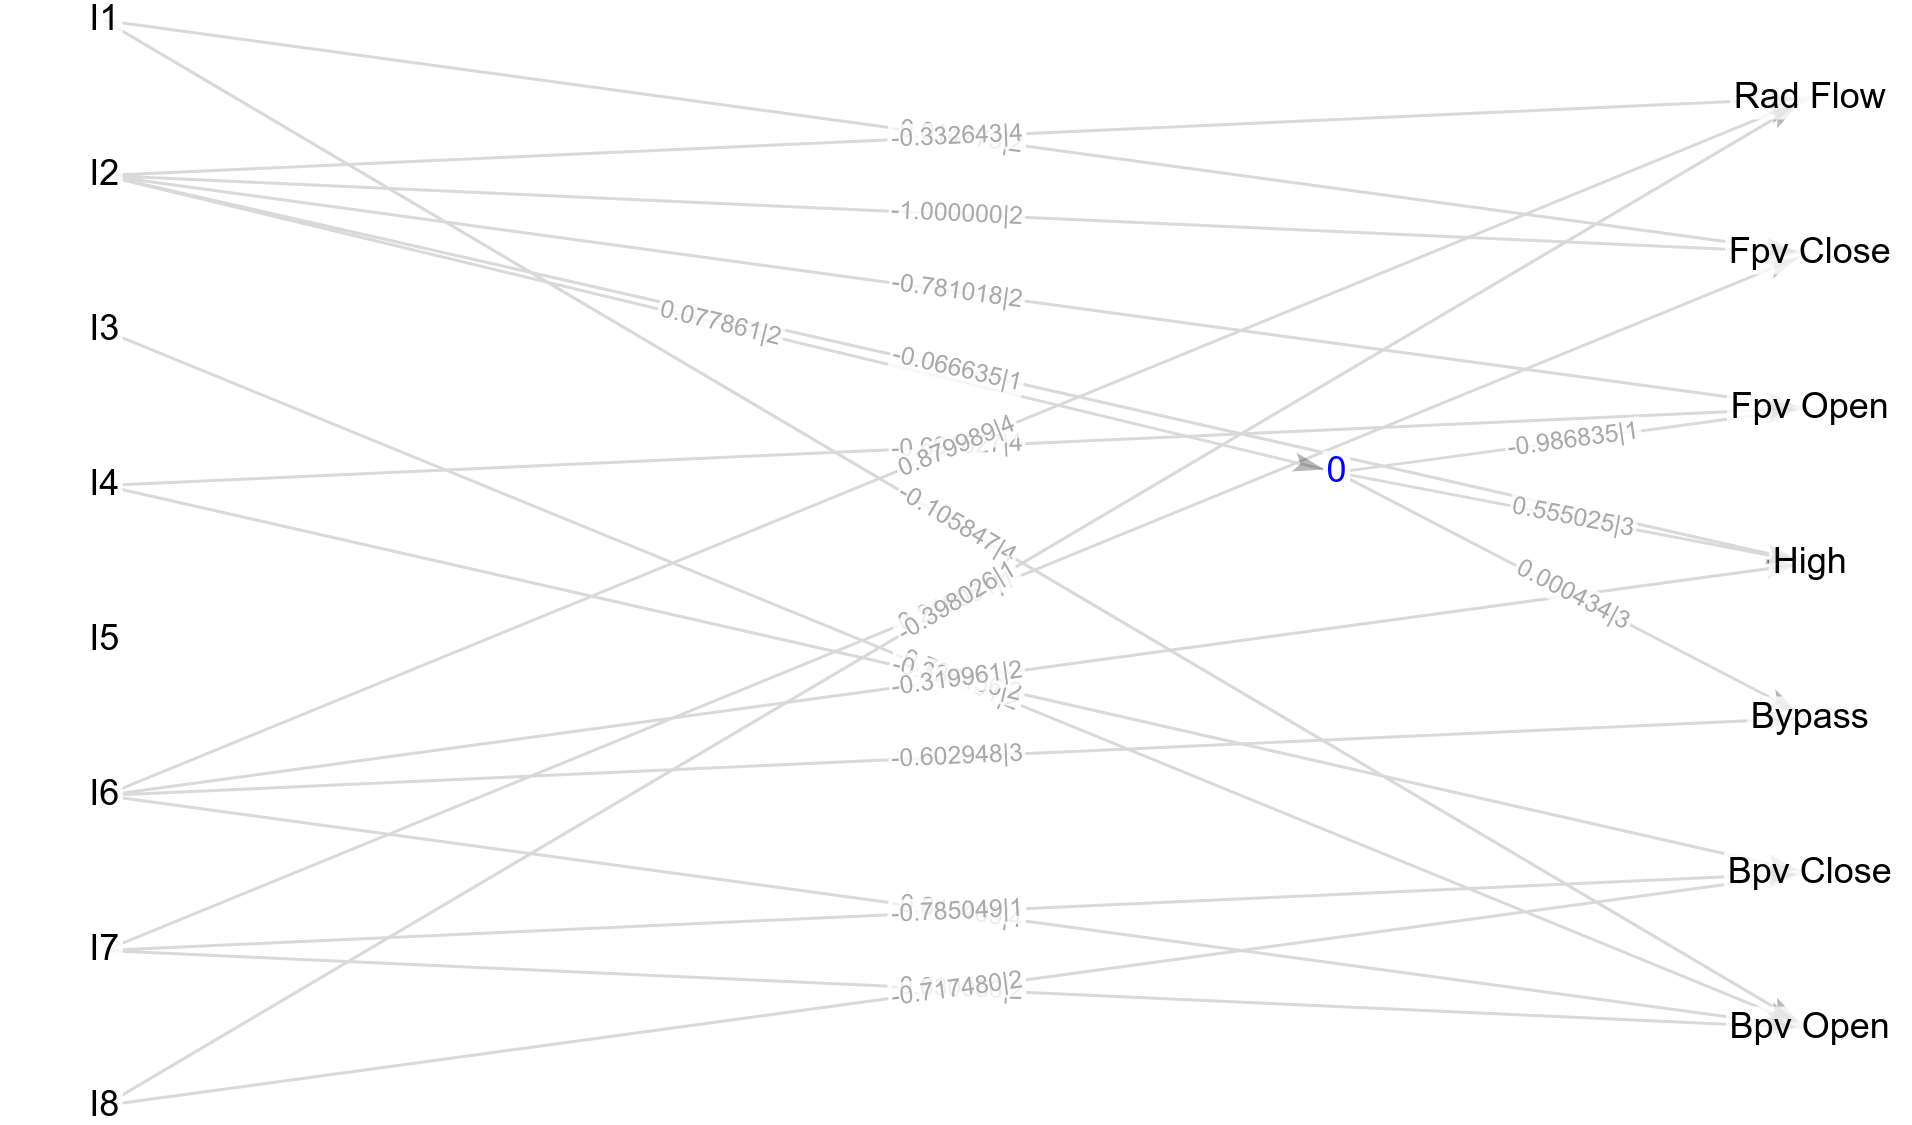
\includegraphics[width=13cm]{shuttle/3/acc_g}
    \end{center}
    \caption{Vizualizacija najbolj točnega agenta tretjega nabora. Vsebuje 1 vmesno vozlišče in 22 povezav.}
    \label{fig:statlog_acc_3_g}
\end{figure}

\begin{figure}[H]
    \begin{center}
        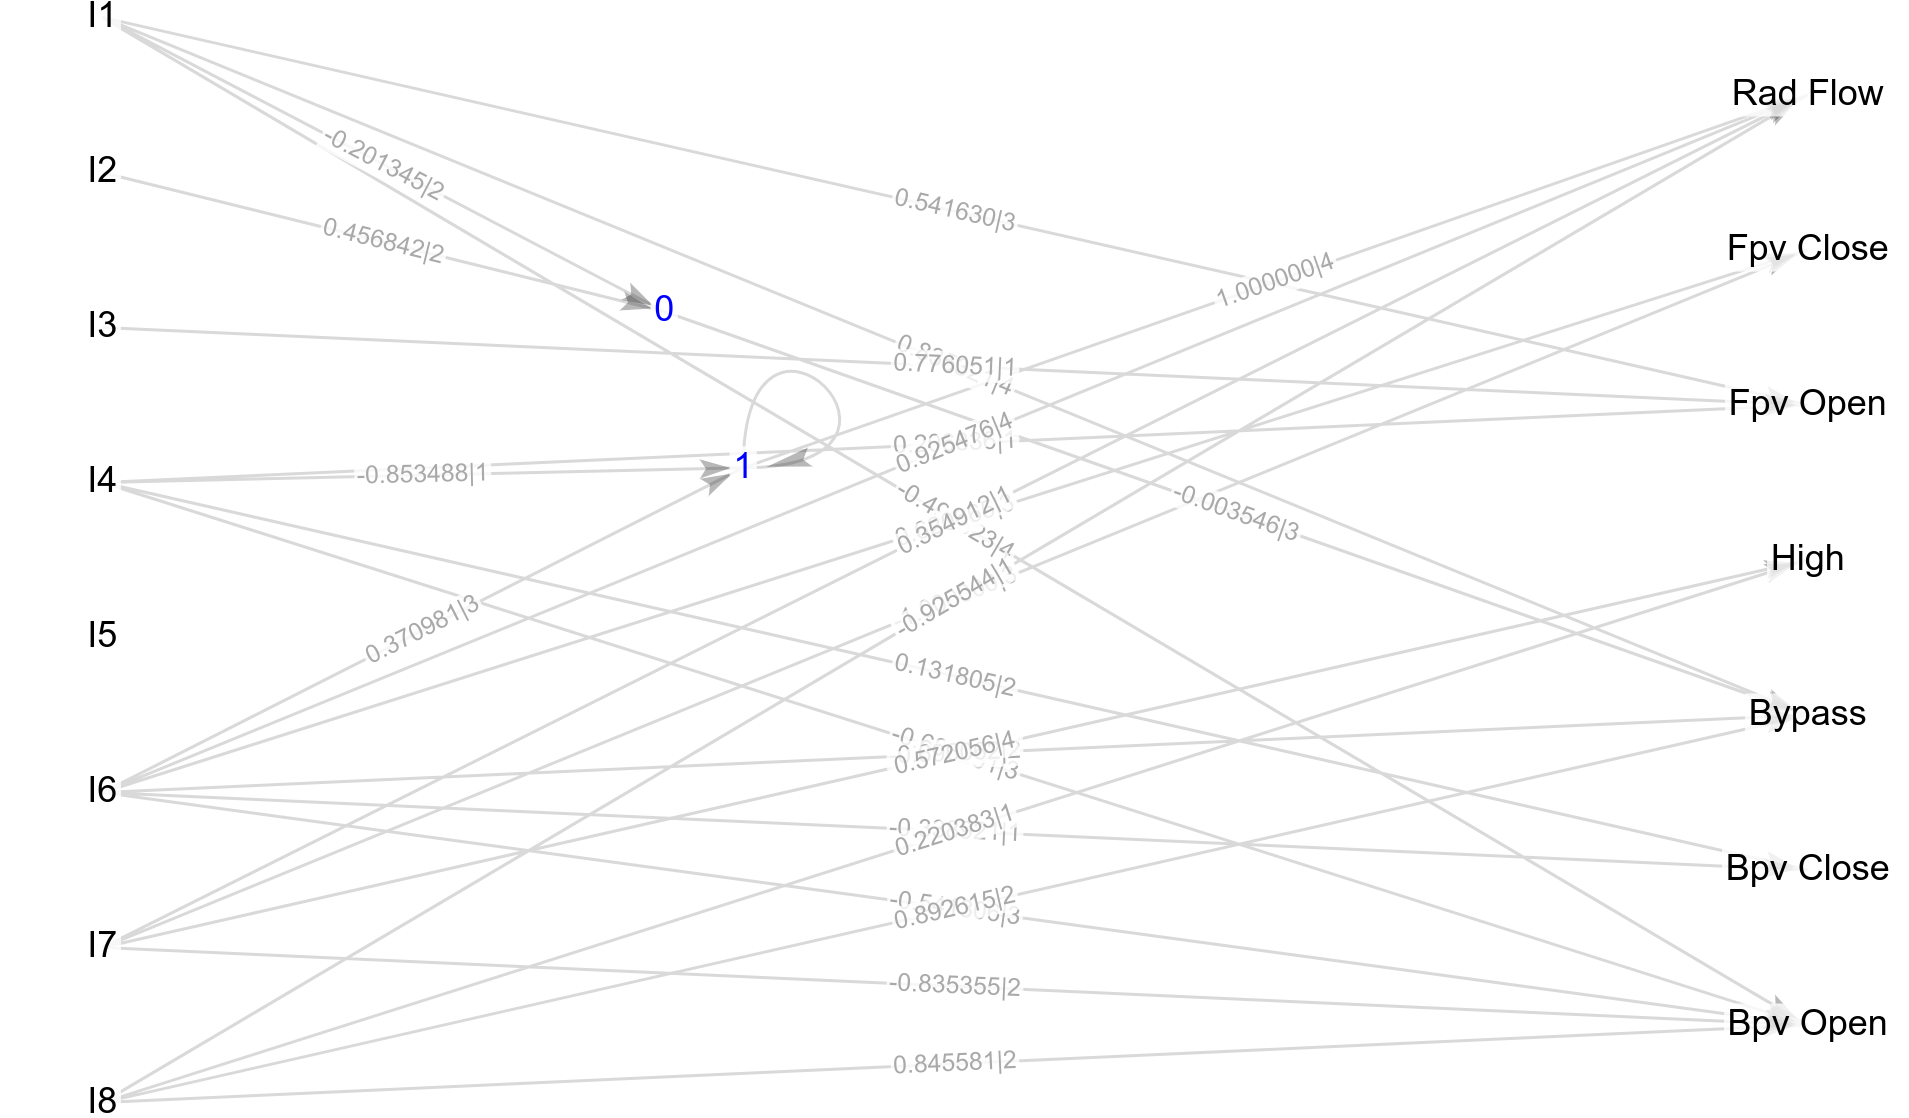
\includegraphics[width=13cm]{shuttle/3/mcc_g}
    \end{center}
    \caption{Vizualizacija agenta z največjim MKK tretjega nabora. Vsebuje 2 vmesni vozlišči in 27 povezav.}
    \label{fig:statlog_mcc_3_g}
\end{figure}